% -*-latex-*-
%\documentclass[handout]{beamer}
\documentclass[12pt]{beamer}
\usepackage{etex}

\let\latexput\put
\usepackage{pictex}
\let\pictexput\put
\let\put\latexput

\usepackage{graphicx,mathdots}
\setbeamertemplate{footline}[frame number]
\setbeamercovered{transparent}
\author{Alan R. Rogers}
\date{\today}
%\UseRawInputEncoding
\begin{document}

\title{Fitness and Inbreeding}
\frame{\titlepage}

\begin{frame}
\frametitle{What inbreeding depression tells us}
\begin{columns}
\column{0.6\textwidth}
 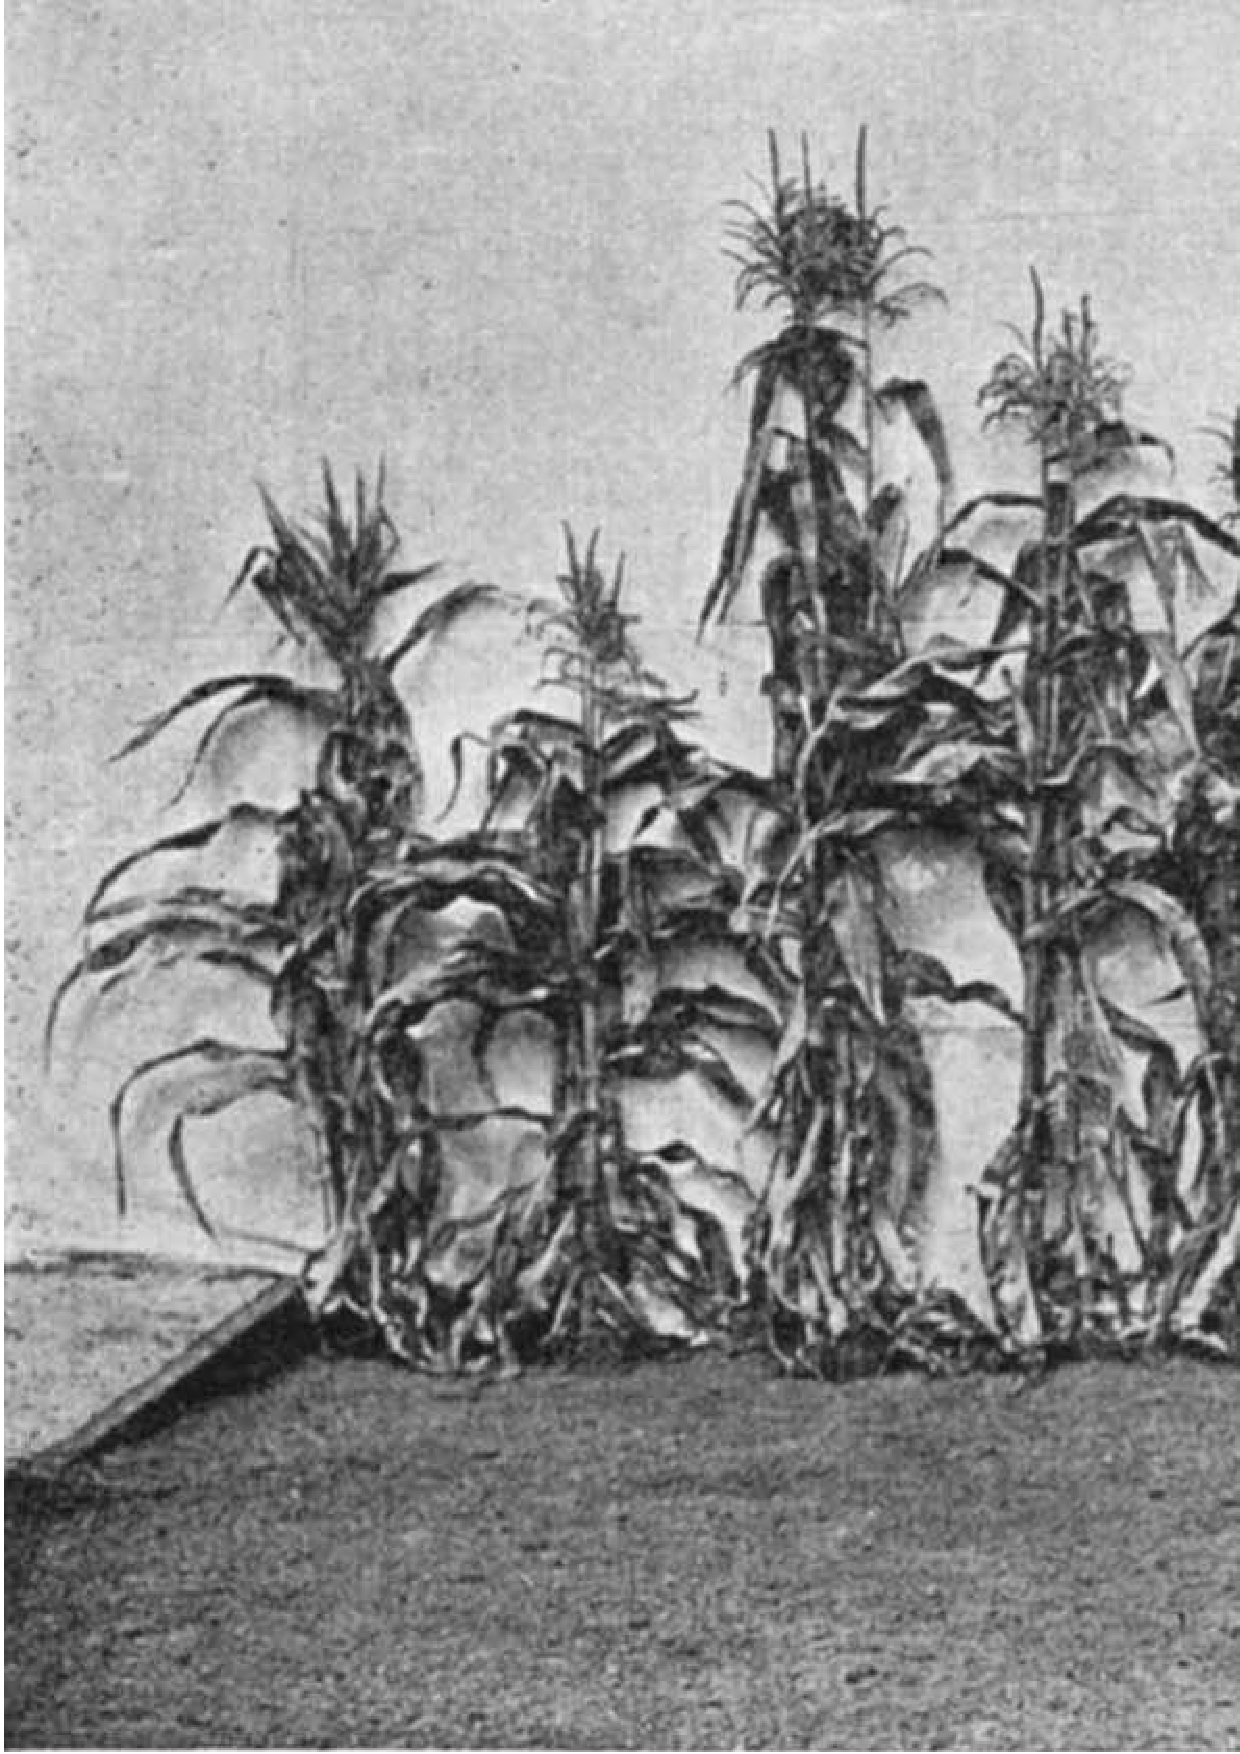
\includegraphics[width=\textwidth]{corn.png}\\
\mbox{}\hfill\textsc{\footnotesize (Jones 1924)}
\column{0.4\textwidth}\raggedright
Inbreeding depression is widespread in Nature.

\bigskip
Implies that deleterious alleles tend to be partially recessive,

\bigskip
or that there is widespread overdominance in fitness.
\end{columns}
\end{frame}

\begin{frame}
\frametitle{Measuring the effect}
\begin{columns}
\column{0.5\textwidth}
\includegraphics[height=0.85\textheight]{mortoncrow.pdf}
\column{0.5\textwidth}
\begin{flushright}
Survival of human children declines with their inbreeding coefficient.

\bigskip

Cousin mating $\Rightarrow F = 0.0625$.

\bigskip

Morton, Crow, and Muller (1956) built a model to estimate this effect.
\end{flushright}
\end{columns}
\end{frame}

\begin{frame}
\frametitle{Genotype frequencies and fitnesses}
\[
\begin{array}{lll}
\hbox{Genotype} & \hbox{Frequency} & \hbox{Fitness}\\
\hline
A_1 A_1 & p^2 + pqF & 1\\
A_1 A_2 & 2pq(1-F)      & 1-hs\\
A_2 A_2 & q^2 + pqF & 1-s\\
\end{array}
\]
\pause
Mean fitness:
\begin{eqnarray*}
\bar w &=& 1 - 2pq(1-F)hs - (q^2 + pqF)s\\
  &=& 1 - a - bF \qquad \Leftarrow \qquad \hbox{linear func of $F$}
\end{eqnarray*}
where
\begin{eqnarray*}
a &=& 2pqsh + q^2s\\
b &=& 2pqs(1/2 - h)
\end{eqnarray*}
\end{frame}

\begin{frame}
\frametitle{Why is inbreeding harmful?}
We have just seen that mean fitness is
\[
\bar w = 1 - a - bF
\]
where
\[
b = 2pqs(1/2 - h)
\]
Fitness decreases with inbreeding if $b>0$, which is true if $s>0$ and
$h<1/2$, or in other words, if deleterious alleles are at least
partially recessive.

\bigskip
If $h < 0$, then heterozygotes have higher fitness than either
homozogte---the case of \emph{overdominance}. Fitness declines with
inbreeding in this case too, because $b>0$.

\bigskip

Inbreeding depression is consistent with either hypothesiss.
\end{frame}

\begin{frame}
\frametitle{Model of Morton, Crow, and Muller}
\begin{columns}
\column{0.5\textwidth}
\textbf{Model}
\begin{eqnarray*}
S &=& \Pr[\hbox{survival}]\\
  &=& \prod_{i=1}^{L} 1 - a_i - b_i F\\
  &\approx& \prod_{i=1} e^{ - a_i - b_i F}\\
  &=& e^{-A - BF}\\
\end{eqnarray*}
where $A=\sum a_i$ and $B = \sum b_i$.
\column{0.5\textwidth}
\pause
\textbf{Estimates}
\begin{eqnarray*}
\hat A &=& 0.1612\\
\hat B &=& 1.734
\end{eqnarray*}

\bigskip
\pause
\textbf{Example}\\
For mating between full sibs, $F=1/4$, and
\begin{eqnarray*}
S &=& \exp\{-0.1612 - 1.734/4\}\\
 &=& 0.85
\end{eqnarray*}
So we expect 15\% mortality in the offspring of full-sib matings.
\end{columns}
\end{frame}

\begin{frame}
  \frametitle{Discussion}
  Inbreeding reduces fitness if $h<1/2$ at the average locus.

  \bigskip

  This is true if deleterious alleles tend to be recessive or if there
  is heterozygote advantage ($h < 0$).

  \bigskip

  Morton, Crow, and Muller did a ``genome-wide'' analysis long before
  there were genome-scale data.
\end{frame}  

\title{Inbreeding and Genetic Drift}
\frame{\titlepage}

\begin{frame}{Inbreeding and drift}

Even under random mating, there is inbreeding in any finite
population.

\bigskip

This ``random inbreeding'' is the same thing as genetic drift.
\end{frame}

\begin{frame}
\frametitle{Number of ancestors}
\centering\begin{tabular}{rrr}
generation   &   year &     ancestors\\
\hline
         0   &   1994 &             1\\
         1   &   1965 &             2\\
         2   &   1936 &             4\\
         3   &   1907 &             8\\
         4   &   1878 &            16\\
         5   &   1849 &            32\\
         6   &   1820 &            64\\
         7   &   1791 &           128\\
         8   &   1762 &           256\\
         9   &   1733 &           512\\
        10   &   1704 &          1,024\\
        11   &   1675 &          2,048\\
        12   &   1646 &          4,096\\
        13   &   1617 &          8,192\\
        14   &   1588 &         16,384\\
\end{tabular}\\
\end{frame}

\begin{frame}
\frametitle{Number of ancestors: II}
\centering\begin{tabular}{rrr}
generation   &   year &     ancestors\\
\hline
        15   &   1559 &         32,768\\
        16   &   1530 &         65,536\\
        17   &   1501 &        131,072\\
        18   &   1472 &        262,144\\
        19   &   1443 &        524,288\\
        20   &   1414 &       1,048,576\\
        21   &   1385 &       2,097,152\\
        22   &   1356 &       4,194,304\\
        23   &   1327 &       8,388,608\\
        24   &   1298 &      16,777,216\\
        25   &   1269 &      33,554,432\\
        26   &   1240 &      67,108,864\\
        27   &   1211 &     134,217,728\\
        28   &   1182 &     268,435,456\\
\end{tabular}\\
\end{frame}

\begin{frame}
\frametitle{Number of ancestors: III}
{\centering
\begin{tabular}{rrr}
generation   &   year &     ancestors\\
\hline
        29   &   1153 &     536,870,912\\
        30   &   1124 &    1,073,741,824\\
        31   &   1095 &    2,147,483,648\\
        32   &   1066 &    4,294,967,296\\
\end{tabular}\\[2ex]}

If you were born in 1994, then you had over 4~billion ancestors in
1066.

\bigskip

But there were not that many people on the planet.

\bigskip

Many of your ancestors in 1066 were the same people---we are all
inbred.

\bigskip
\pause

Let us build a model of this inbreeding.
\end{frame}

\begin{frame}
\frametitle{Drift and inbreeding}

\textbf{Drift} After $t$ generations of genetic drift, the expected
heterozygosity is
\[
E[H(t)|p_0] =2p_0q_0 (1 - 1/2N)^t
\]

\textbf{Inbreeding} If $F_t$ is the average inbreeding coefficient in
generation $t$, relative to generation~0,
\[
E[H(t)|p_0] = 2p_0q_0 (1 - F_t)
\]

Equating these expressions gives
\[
F_t = 1 - (1-1/2N)^t
\]
Inbreeding \emph{is} genetic drift.
\end{frame}

\end{document}

